
\documentclass[a4paper,10pt,english]{article}
\usepackage[utf8]{inputenc}
\usepackage[english]{babel}

\usepackage{amsmath,graphicx,varioref,verbatim,amsfonts,geometry}
\usepackage[thinc]{esdiff}
\usepackage[usenames,dvipsnames,svgnames,table]{xcolor}
\usepackage[colorlinks=false]{hyperref}

\usepackage{bm}

\setlength{\parindent}{0mm}
\setlength{\parskip}{1.5mm}

\usepackage{textcomp}
\definecolor{listinggray}{gray}{0.9}
\definecolor{lbcolor}{rgb}{0.9,0.9,0.9}

\usepackage{listings}

\lstdefinelanguage{python}
{
	morekeywords={print,abs,for,def,if,while,do,break,return,from,import,try,except,else,elif},
	sensitive=false,
	morecomment=[l]{\#}
}

\lstset{language=python,
	backgroundcolor=\color[rgb]{.95,.95,.95},
	numbers=left,xleftmargin=10pt,
	numberstyle=\tiny,stepnumber=1,numbersep=5pt,
	stringstyle=\color{red},
	basicstyle=\footnotesize \ttfamily,
	keywordstyle=\color{blue},
	commentstyle=\color{green},
	basewidth=0.60em,
	showstringspaces=false,
	captionpos=b,
	frame=single
}

\newcounter{subproject}
\renewcommand{\thesubproject}{\alph{subproject}}
\newenvironment{subproj}{
\begin{description}
\item[\refstepcounter{subproject}(\thesubproject)]
}{\end{description}}

%Lettering instead of numbering in different layers
% \renewcommand{\labelenumi}{\alph{enumi}}
\renewcommand{\thesubsection}{\alph{subsection}.}

\title{MAT1110 - Mandatory assignment 1}
\author{William Dugan}

\begin{document}

\maketitle

\section{}

\subsection{}
The curve $C$ is given the following parametrisation:
\begin{align}
    \bm{r}(t) = 
        \left( 
            a \cdot \text{arcsinh} \left( 
                                \frac{t}{a}
                            \right),
            \sqrt{t^2+a^2}
        \right)
\end{align}
for $-b \leq t \leq b$. $\bm{r}'(t)$ is
\begin{align*}
    \bm{r}'(t) 
    &= 
        \left( 
            \frac{a}{\sqrt{1 + {\left( \frac{t}{a} \right)}^2}} \cdot \frac{1}{a},
            \frac{1}{2\sqrt{t^2+a^2}} \cdot 2t
        \right) \\
    &= \left( 
            \frac{a}{\sqrt{t^2+a^2}},
            \frac{t}{\sqrt{t^2+a^2}}
        \right).
\end{align*}
Its length is
\begin{align*}
    ||\bm{r}'(t)||
    =& 
        \sqrt{
            \left(
                \frac{a}{\sqrt{t^2+a^2}}
            \right)^2
            +
            \left(
                \frac{t}{\sqrt{t^2+a^2}}
            \right)^2
        } \\
    &= 
        \sqrt{
            \frac{a^2+t^2}{a^2+t^2}
        } \\
    &= 1
\end{align*}

\subsection{}
The length of a curve is given by
\begin{align}
    s = \int_a^b v(t) dt = \int_a^b ||\bm{r}'(t)|| dt
\end{align}
Hence, the length of $C$ is
\begin{align*}
    s &= \int_{-b}^{b} dt = 2b
\end{align*}

\newpage
\subsection{}
See python code at the end of the paper.
\vspace{-1cm}
\begin{figure}[h]
    \centering
    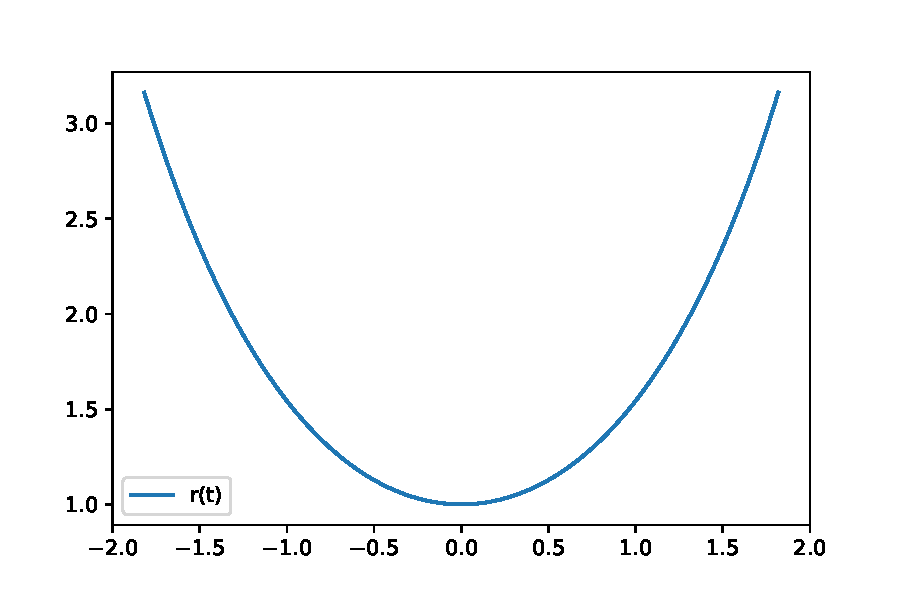
\includegraphics[
        scale=0.8]{figure1.pdf}
    \caption{Plot of the catenary curve using $a=1, b=3$}
    \label{fig:fig1}
\end{figure}

\subsection{}
\begin{align}
    \rho_t 
    &= \frac{\partial\rho}{\partial t}
    = \left(
        \frac{a}{\sqrt{t^2+a^2}},
        \frac{t}{\sqrt{t^2+a^2}} \cos\theta,
        \frac{t}{\sqrt{t^2+a^2}} \sin\theta
    \right) \\
    \rho_\theta 
    &= \frac{\partial\rho}{\partial\theta}
    = \left(
        0,
        -\sqrt{t^2+a^2} \sin\theta,
        \sqrt{t^2+a^2} \cos\theta
    \right)
\end{align}    


We define the surface unit normal as
\begin{align*}
    \bm{n} = \frac{\bm{f}}{f}
\end{align*}
where $\bm{f} = \rho_t \times \rho_\theta$ and $f = ||\bm{f}||$. Taking the cross product of $\rho_t$ and $\rho\theta$ gives
\begin{align*}
    \bm{f} = 
        \left(
            t, 
            -a \cdot\cos\theta, 
            -a \cdot\sin\theta
        \right)
\end{align*}
which has a length
\begin{align*}
    f 
    &= ||\bm{f}|| \\
    &= \sqrt{
        t^2 + (-a)^2 \cdot (\cos\theta + \sin\theta)
    } \\
    &= \sqrt{
    t^2 + a^2
    }
\end{align*}
Hence the surface unit normal $\bm{n}$ is
\begin{align}
    \bm{n} 
    = \frac{\bm{f}}{f}
    = 
    \left(
        \frac{t}{\sqrt{t^2 + a^2}},
        - \frac{a \cot\cos\theta}{\sqrt{t^2 + a^2}},
        - \frac{a \cdot\sin\theta}{\sqrt{t^2 + a^2}}
    \right)
\end{align}

\subsection{}
We define the following:
\begin{align*}
    &E = ||\rho_t||^2,
    &&F = \rho_t\cdot\rho_\theta,
    &&&G = ||\rho_\theta||^2 \\
    &L = \rho_{tt}\cdot\bm{n},
    &&M = \rho_{t\theta}\cdot\bm{n},
    &&&N = \rho_{\theta\theta}\cdot\bm{n}
\end{align*}
The mean curvature of a surface $S$ is given by
\begin{align}
    H = \frac{1}{2} \frac{EN - 2FM + GL}{EG - F^2}
\end{align}
and $S$ is a minimal surface if $H=0$ at all points. For this to be true, the numerator has to be zero for all $t$. Since $\rho_t$ and $\rho_\theta$ is normal to each other, $F=0$, hence $-2FM=0$. We need $EN-GL=0$.
\begin{align*}
    E &= 
        \sqrt{
            \frac{a^2}{t^2+a^2} 
            + \frac{t^2 \cdot\cos^2\theta}{t^2+a^2}
            + \frac{t^2 \cdot\sin^2\theta}{t^2+a^2}
        }
        = 1 \\
    G &= 
        {\sqrt{
        (t^2+a^2)\cdot\sin^2\theta + (t^2+a^2)\cdot\cos^2\theta
        }}^2
        = t^2+a^2 \\
    L &=
        - \frac{a\cdot t^2}{(t^2+a^2)^2}
        - \frac{a^3\cdot\cos^2\theta}{(t^2+a^2)^2}
        - \frac{a^3\cdot\sin^2\theta}{(t^2+a^2)^2}
        = - \frac{a}{t^2+a^2} \\
    N &= 
        a\cdot\cos^2\theta + a\cdot\sin^2\theta 
        = a \\
\end{align*}
If we put this together, we get
\begin{align*}
    1\cdot a - (t^2+a^2) \cdot \frac{a}{(t^2+a^2)} = 0
\end{align*}
and $S$ is a minimal surface.

\newpage
\section{}
\begin{align*}
    \bm{F}(x, y) &= (ax+by, cx+dy) \\
    \bm{F^\perp}(x, y) &= (-cx-dy, ax+by) \\
    \phi (x, y) &= -\frac{c}{2}x^2 + axy + \frac{b}{2}y^2
\end{align*}

\subsection{}
$\bm{F}$ and \bm{$F^\perp$} are orthogonal if the dot product between them is zero.
\begin{align*}
    (ax+by)(-cx-dy) + (xc+dy)(ax+by) = 0.
\end{align*}

\subsection{}
For any field $\bm{F}$ to be conservative, the following condition must be true for all $\Vec{x}, i, j$:
\begin{align}
    \frac{\partial \bm{F}_i}{\partial x_j} (\Vec{x})
    = \frac{\partial \bm{F}_j}{\partial x_i} (\Vec{x})
\end{align}

In our case we have
\begin{align*}
    &\frac{\partial \bm{F_1^\perp}}{\partial y} = -d, 
    &&\frac{\partial \bm{F_2^\perp}}{\partial x} = a
\end{align*}
Hence, $\bm{F^\perp}$ is conservative when $d=-a$. Furthermore,
\begin{align*}
    \nabla\phi (x, y)
    &= \left( 
        -cx+ay,
        ax+by
    \right) \\
    &= \left( 
        -cx-dy,
        ax+by
    \right) \\
    &= \bm{F^\perp}
\end{align*}

\subsection{}
We use the parametrisation $\bm{r}(t)=(x(t), y(t))$. This gives $\phi(x, y) = \phi(\bm{r}(t))$. The contours of $\bm{F}$ is given when $\phi(\bm{r}(t))$ is constant. This gives
\begin{align*}
    \diff{}{t} \phi(\bm{r}(t)) &= 0 \\
    \nabla\phi(\bm{r}(t)) \cdot (\bm{r}'(t)) &= 0
\end{align*}
which shows that $\nabla\phi$ is perpendicular to the contour lines. 

\newpage
\subsection{}
Since the contour lines to $\phi$ is perpendicular to $\bm{F^\perp}$ (as we found in the previous task), and $\bm{F^\perp}$ is perpendicular to $\bm{F}$, the contour lines are parallel with $\bm{F}$. This means that the contour lines are tangential to $\bm{F}$ and gives the field lines for the vector field$\bm{F}$.

\subsection{}
\vspace{-1cm}
\begin{figure}[h]
    \centering
    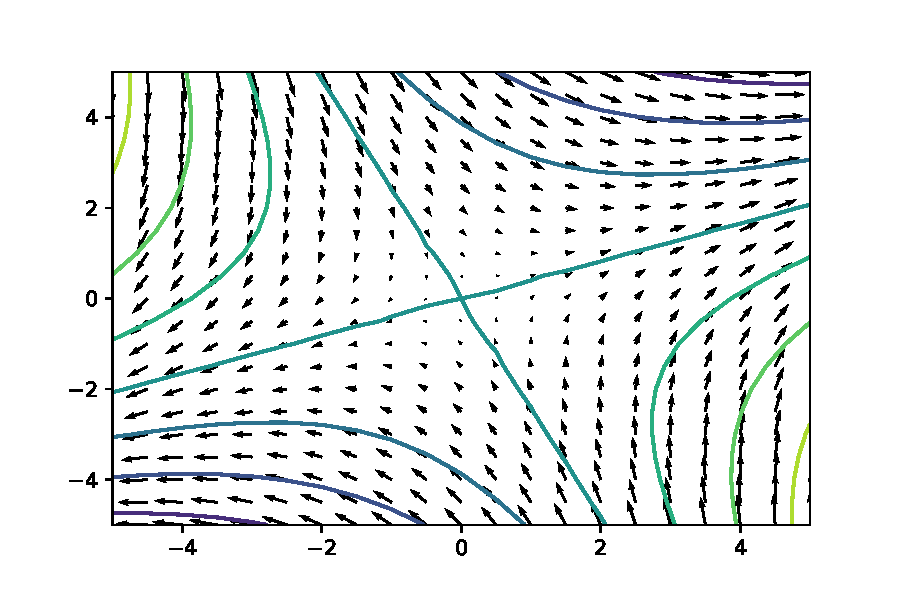
\includegraphics[scale=0.8]{figure2.pdf}
    \caption{Plot of vector field $\bm{F}$ and its contour lines. $a=b=c=1$.}
    \label{fig:fig2}
\end{figure}
\vspace{-1cm}
\begin{figure}[h!]
    \centering
    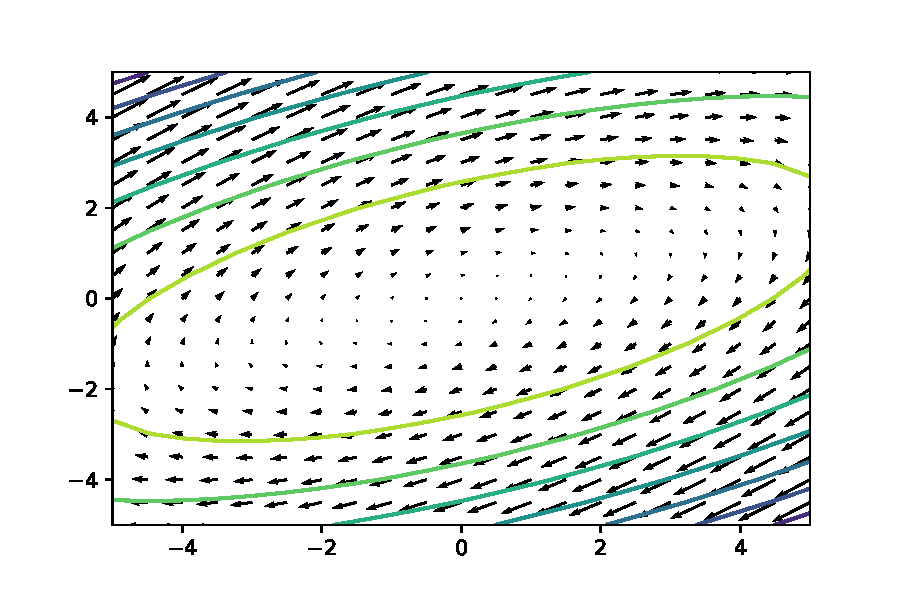
\includegraphics[scale=0.8]{figure3.pdf}
    \caption{Plot of vector field $\bm{F}$ and its contour lines. $a=-1, b=3, c=-1$.}
    \label{fig:fig3}
\end{figure}

\newpage
\section*{Python code}
\begin{lstlisting}
import numpy as np
import matplotlib.pyplot as plt

a = 1
b = 3

t = np.linspace(-b, b, 1001)
r = np.asarray([a*np.arcsinh(t/a), np.sqrt(t**2+a**2)])

plt.plot(r[0], r[1], label='r(t)')
plt.legend()
plt.show()

for a, b, c in ((1, 1, 1), (-1, 3, -1)):
    plt.clf()
    d = -a

    t = np.linspace(-5, 5, 21)
    x, y = np.meshgrid(t, t)

    u, v = a*x + b*y, c*x + d*y
    phi = c*x**2 - 2*a*x*y - b*y**2

    plt.quiver(x, y, u, v)
    plt.contour(x, y, phi)
    plt.show()
\end{lstlisting}

\end{document}
